\documentclass{article}
\usepackage[utf8]{inputenc}

\title{CS 376 : HW 4 - Continuous Systems}
\author{Fred Eisele }
\date{15 October 2014 }

\usepackage{natbib}
\usepackage{graphicx}
\usepackage{tikz}
\usetikzlibrary{shapes,arrows}
\usepackage{amsmath}
\usepackage{amsfonts}
\usepackage{xfrac}

\begin{document}

\maketitle

This problem set is taken from \citep{IntroEmbedSys} chapter 2 : Problem 6.
This system makes use of a helicopter model,
Figure \ref{fig:helicopter_plant}.

\begin{figure}[h!]
\centering
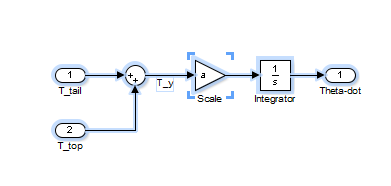
\includegraphics[scale=0.8]{helicopter_model.png}
\caption{the helicopter plant model (SimuLink)}
\label{fig:helicopter_plant}
\end{figure}

This Simulink model corresponds to the following mathematical model.

\begin{equation}
\forall t \in \mathbb{R} ,  \qquad
y_1(t) = a x_1(t)
\end{equation}

\ldots and for the Integrator \ldots
\begin{equation}
\forall t \in \mathbb{R},  \qquad
y_2(t) = i + \int_0^t x_2(\tau) \, \mathrm{d}\tau
\end{equation}

The following expresses the mapping to the helicopter model.
Notice that the memory carrying element in the models is the integrator in all cases.

\begin{align}
a & = \frac{1}{I_{yy}} & \text{characteristic of the helicopter} \in \mathbb{R}_+ \\
i & = \dot{\theta}(0) = 0 & \text{initial \emph{resting} angular velocity} \\
x_i & = T_y        & \text{total y torque} \in \mathbb{R} \\
y_2 & = \dot{\theta} & \text{output angular velocity} \\
y_1 & = x_2   &  \text{cascade composition} \\
T_{tail} &  \text{  follows  } T_{top}
\end{align}
The tail-rotor torque compensates for the top-rotor torques.

Using Simulink and its continuous-time modeling component
I have built a model of the helicopter control
system shown in Figure \ref{fig:control_system}.
This model has an upper section that models a system
with a proportional (P)-controller and a lower section
that models a proportional-integrator (PI)-controller.
The P-controller subsystem illustrates problem a)
with the lower PI-controller subsystem illustrates problem b).
These are placed together so that the inputs and outputs
may be shared and displayed together.
In this model the value of $a = 5$ and $T_top = 4$ are
arbitrarily choosen.


\begin{figure}[h!]
\centering
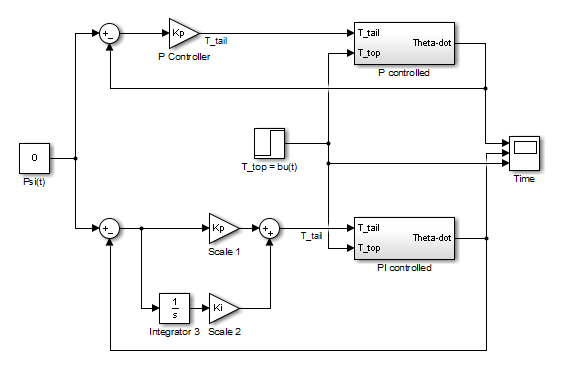
\includegraphics[scale=0.8]{controller_model.png}
\caption{the control systems models (SimuLink)}
\label{fig:control_system}
\end{figure}

\section{P-controller system}

Given some reasonable input parameters the
actual angular velocity, $\dot{\theta}$, is shown
as a function of time.
The initial and operating conditions
specify that the desired angular velocity
is zero, $\phi (t) = 0$, and that the
top-rotor torque is non-zero,
$T_{top}(t) = b u(t) = 4$ moving to that
value as a step function at time $t = 1$.
Given are plots for several values of $K_p$.

\begin{figure}[h!]
\centering
\includegraphics[scale=0.8]{theta_dot_kp_100_ki_12.png}
\caption{$K_p = 100, K_i = 12$}
\label{fig:td_100_12}
\end{figure}

\begin{figure}[h!]
\centering
\includegraphics[scale=0.8]{theta_dot_kp_40_ki_12.png}
\caption{$K_p = 40, K_i = 12$}
\label{fig:td_40_12}
\end{figure}

\begin{figure}[h!]
\centering
\includegraphics[scale=0.8]{theta_dot_kp_30_ki_12.png}
\caption{$K_p = 30, K_i = 12$}
\label{fig:td_30_12}
\end{figure}

Once the $T_{top}$ has changed a new stable but
typically non-zero $\dot{\theta}$ is approached asymtotically
(from the text the value approached is $b/K_p$).
The value of the new \dot{theta} follows $K_p$ as can be
observed from the progression Figure \ref{fig:td_100_12}
\rightarrow Figure \ref{fig:td_40_12} \rightarrow Figure \ref{fig:td_30_12}.


\begin{figure}[h!]
\centering
\includegraphics[scale=0.8]{theta_dot_kp_30_ki_12k.png}
\caption{$K_p = 30, K_i = 12$}
\label{fig:td_30_1200}
\end{figure}

The Figure \ref{fig:td_30_1200} illustrates the convergence.


\section{PI-controller system}
The lower portion of Figure \ref{fig:control_system}
replaces the proportional (P) controller of the upper system
with a propotional-integrator (PI) controller.
This alternative controller has an additional parameter
associated with the intgrator, $K_i$.
Experiment with this new value shows that the
error is corrected for over time,
recalling that the integrator has memory.

\begin{figure}[h!]
\centering
\includegraphics[scale=0.8]{theta_dot_kp_30_ki_120.png}
\caption{$K_p = 30, K_i = 120$}
\label{fig:td_30_120}
\end{figure}

\begin{figure}[h!]
\centering
\includegraphics[scale=0.8]{theta_dot_kp_30_ki_24.png}
\caption{$K_p = 30, K_i = 24$}
\label{fig:td_30_24}
\end{figure}

A larger value of $K_i$ can be observed to cause a
more rapid asymptotic convergence of
$\dot{\theta}$ to the control-value, $\Psi = 0$
after $T_{top}$ changes.
This behavior can be seen by comparing
Figure \ref{fig:td_30_120} to Figure \ref{fig:td_30_24}
where $K_p$ is held constant and $K_i$ is changed.


\bibliographystyle{plain}
\bibliography{references}
\end{document}
